% The master file for the thesis. Compile it for entire thesis creation.

% Select document class first
\documentclass{scrbook}

\KOMAoptions{
    paper=a4,
    fontsize=12pt,
    DIV=12,
    BCOR=0mm,
    twoside=off,
    index=totoc,
    listof=totoc,
}

% Import the doc with packages and other settings
% !TEX root = ../main.tex

%%%%%%%%%%%%%%%%%%%%%%%%%%%%%%%%%%%%%%%%%%%%%%%%%%%%%%%%%%%%%%%%%%%%%
% LaTeX preamble where all required packages and macros can be defined. 
% This needs to be done before the \begin{document} command.

% Font encodings
\usepackage[TS1,T1]{fontenc}

% UNICODE recognition:
% This package should recognise any UNICODE characters in the text and automatically replace them with their standard macros
\usepackage[utf8]{inputenc}

% Graphics package and path to graphics.
\usepackage{graphicx}
\graphicspath{ {figures/} }

% Sections styles
\usepackage{sectsty}

% AMS maths packages
\usepackage{
    amsmath,
    amsfonts,
    amsthm
}

% Todo notes. Used for notes and annotations.
\usepackage{todonotes}

% Natbib package for text references
\usepackage[
    round,
    super,
    comma,
    sort&compress
]{natbib}
\bibliographystyle{unsrtnat}
\usepackage{natmove}

% For better looking captions.
\usepackage{caption}

% For subfigures
\usepackage{subcaption}

% For float barriers and such
\usepackage{placeins}

% Better tables 
\usepackage{
    booktabs,
    makecell,
    array,
    multirow,
    tabularx
    }

% The SIunitx package enables the \SI{}{} command.
\usepackage{siunitx}

% The mchem package for formula subscripts using \ce{}
\usepackage[version=4]{mhchem} 

% Clickable URL's can be made with this package: \url{}.
\usepackage{url}

% To reference another document, in this case the SI
\usepackage{zref-xr,zref-user}
\zxrsetup{
    tozreflabel=false, 
    toltxlabel=true, 
    verbose
}
%\zexternaldocument*{si}

% This package makes all references clickable. 
% By default, these references become boxed and colored. This is turned back to normal with the \hypersetup command below.
\usepackage{hyperref}

\hypersetup{
    %backref=true,                          %% add links (default)
    %pagebackref=true,                      %% in the bibliography (default)
    %hyperindex=true,                       %% in the index (default)
    %bookmarks=true,                        %% Acrobat bookmarks (default)
    breaklinks=true,                        %% break lines if long
    colorlinks=true,                        %% colour links
    urlcolor=blue,                          %% link colour
    citecolor=blue,	                        %% bibliography link color
    linkcolor=blue,	                        %% internal link color
    anchorcolor=blue,                       %% anchor link color
    bookmarksopen=false,                    %% bookmarks default open
    linktocpage=false,                      %% pagenumber link in TOC
    pdfborder={0 0 0}                       %% pdf border settings
}


% Font settings
%% Title font
%% Bibliography font
\renewcommand{\bibfont}             {\usefont{T1}{bch}{m}{n}\selectfont}

%% Figure legend fonts
%% Legend font
\renewcommand{\captionfont}         {\usefont{T1}{cmbr}{m}{n}\selectfont\small}
%% Label legend font
\renewcommand{\captionlabelfont}    {\usefont{T1}{cmbr}{m}{n}\selectfont}

% Import the doc with the drafting
% !TEX root = ../main.tex

% Setup for drafting
\includeonly{
    chapters/ch2/ch-main,
    backmatter/a1/appx-main,
    backmatter/a2/appx-main,
    backmatter/a4/appx-main,
}


%%%%%%%%%%%%%%%%%%%%%%%%%%%%%%%%%%%%%%%%%%%%%%%%%%%%%%%%%%%%%%%%%%%%%
\begin{document}

% Frontmatter
\frontmatter
% !TEX root = ../main.tex
\begin{titlepage}

\vspace*{-2cm}
\begin{center}
	\begin{minipage}[c]{0.3\linewidth}
		\raggedright
		
\includegraphics[height=2cm]{logo_cnrs}
	\end{minipage}\hfill
	\begin{minipage}[c]{0.3\linewidth}
		\centering
		\includegraphics[height=2cm]{logo_madirel}
	\end{minipage}\hfill
	\begin{minipage}[c]{0.3\linewidth}
		\raggedleft
		\includegraphics[height=2cm]{logo_defnet}
	\end{minipage}\hfill

	\vspace{1.5cm}

	\LARGE \scshape
	Exploring Sources of Variability in Metal Organic Frameworks 
	Through High Throughput Adsorption and Calorimetric Methods \\
	\vspace{1.5cm}
	\Large \upshape 
	Paul-Adrian Iacomi \\
	\vspace{1.8cm}
	\large \upshape
	A thesis submitted with the view of obtaining the degree of \\
	\textit{Doctor of Philosophy}\\

	\vspace{1cm}
	\begin{minipage}[c]{\linewidth}
		\centering
		
\includegraphics[height=2cm]{logo_amu_excellence}
	\end{minipage}\hfill
	\vspace{1.6cm}

\end{center}

\begin{flushleft}
	\vspace{0.2cm}
	\normalsize 
	Doctoral School: \textit{Physics and Material Science}\\
    Discipline: \textit{Material Science}\\
    Specialty: \textit{Characterisation of Porous Materials}\\
	\vspace{0.5cm}
    \normalsize Defended on 15/10/2018 in front of the following jury:\\
\end{flushleft}
\vspace{0.1cm}
\begin{tabular}{lll}
	Rob Ameloot & KU Leuven & Reviewer \\
    \vspace{0.08cm}
	Flor Siperstein & The University of Manchester & Reviewer \\
    \vspace{0.08cm}
	Stefan Kaskel & TU Dresden & Examinator \\
    \vspace{0.08cm}
	Bogdan Kuchta & CNRS/AMU & Examinator \\
    \vspace{0.08cm}
	Philip L. Llewellyn & CNRS/AMU & Thesis director \\
\end{tabular}
\vspace{0.3cm}
\begin{flushleft}\normalsize National thesis number: 2017AIXM0001/001ED62\\\end{flushleft}

\end{titlepage}
% !TEX root = ../main.tex

\newpage
\thispagestyle{empty}

~\vfill
\begin{center}
    \begin{minipage}[c]{0.25\linewidth}
        \raggedright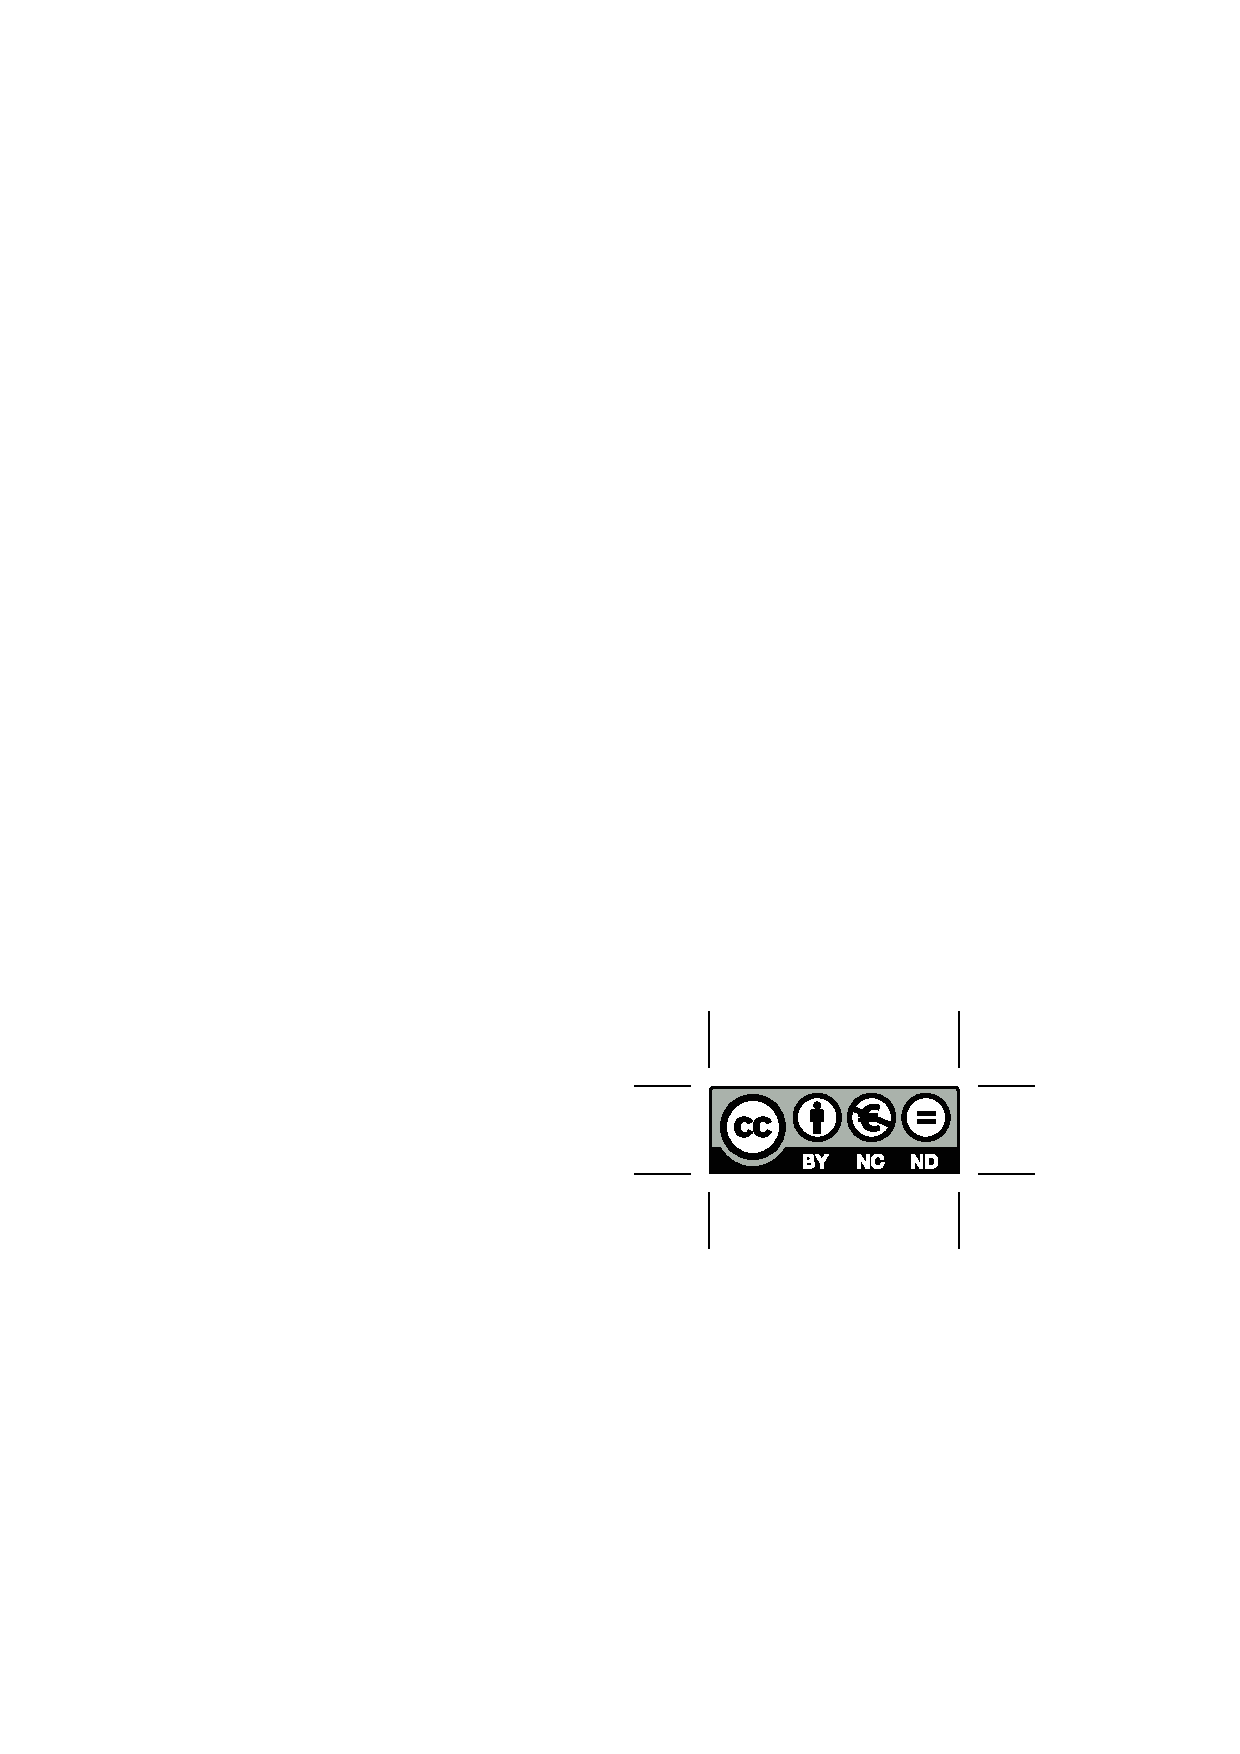
\includegraphics[height=35px]{by-nc-nd-eu}
    \end{minipage}\hfill
\end{center}

\begin{center}
This work falls under the conditions of the 
\href{https://creativecommons.org/licenses/by-nc-nd/4.0}
{%
Creative Commons Attribution License --- No commercial use --- 
No modification 4.0 International}.
\end{center}

% !TEX root = ../main.tex

\chapter{Abstract}

\gls{MOF}s are a class of hybrid porous materials
which has been the focus of much scientific interest since their
discovery in the late 20\textsuperscript{th} century. These
coordination polymers consist of three-dimensional networks of 
metal nodes interlinked by polytopic organic molecules. Their 
potential stems from the possible rational design
of \gls{MOF}s for highly efficient or unique applications. 
With judicious choice of building blocks, the framework can be used for
carbon dioxide capture from air, hydrogen storage or regioselective 
catalysis. Furthermore, taking advantage of specific properties such 
as flexibility, magnetism or photoelectrics may even result in 
their use in drug delivery, micro mechanical devices,
sensors and optoelectronics.

However, their properties also introduce significant difficulty
in \gls{MOF} adsorption characterisation.
Structural defects, crystal size, shaping procedure
and the aforementioned flexible behaviour can lead to irreproducibility 
in isotherms. The first step to ensuring consistent results
is to ensure that a common framework of processing methods is 
established. In this thesis, the creation of an open-source codebase
is detailed, which is intended to standardize the processing of 
isotherms. Using this framework, high throughput processing of more
than 18 000 isotherms is used to explore the scale of uncertainty 
present in published adsorption data.
The focus turns towards using complementary methods to extend the
high throughput methodology through advanced characterisation.
Direct measurement of the differential enthalpy of adsorption
using \textit{in situ} microcalorimetry is shown to be an excellent
avenue of obtaining further insight into the contribution of material, 
guest-host and host-host interactions to the overall energetics of
adsorption.

Together, these methods are used to study some of the sources 
of the variability of \gls{MOF}s, and quantify their effect.
First, the impact of structural defects is investigated, through an
alternative post-synthetic method of missing linker/cluster generation
in the prototypical UiO-66(Zr) \gls{MOF}. The processing of 
materials for their use in an industrial environment through 
shaping is another potential source of performance modification,
which is here studied as the effect of wet granulation on
three topical \gls{MOF}s (UiO-66(Zr), MIL-100(Fe) and MIL-127(Fe)). 
Finally, counterintuitive behaviours intrinsic to
``soft'' porous crystals are detailed, where the structure itself 
is responsible for fluctuation in adsorption isotherms. Here,
a fundamental study on a copper paddlewheel based material, DUT-49(Cu)
yields know-how on the source of adsorption induced compliance
and its tunability through structural modification.

\pagebreak

\chapter{Résumé}

Les réseaux métallo-organiques (MOF) sont une classe de matériaux poreux
hybrides qui ont suscité un grand intérêt scientifique depuis leur 
découverte à la fin du 20ème siècle. Ces polymères de coordination sont 
constitués de réseaux tridimensionnels de nœuds métalliques interconnectés 
par des molécules organiques polytopiques. L'intérêt pour ces matériaux 
provient de la conception rationnelle possible des MOF pour des 
applications hautement efficaces ou uniques.
Leur flexibilité, magnétisme ou effet photoélectrique
peut même conduire à leur utilisation dans l'adsorption et stockage du
gas, catalyse, délivrance de médicaments, des dispositifs micro-mécaniques
ou des capteurs.

Cependant, leurs propriétés uniques introduisent également des difficultés
significatives dans la caractérisation par adsorption de gaz, avec les 
défauts structurels, la taille des cristaux, la procédure de mise en forme et le 
comportement flexible susmentionné comme un example. 
La première étape pour obtenir des résultats reproductibles consiste à s'assurer
qu'un cadre commun de méthodes de traitement 
est établi. Dans cette thèse, la création d'un code source libre est détaillé, 
pour standardiser le traitement des isothermes. En utilisant, un traitement à 
haut débit de plus de 18 000 isothermes est 
utilisé pour explorer l'échelle d'incertitude présente dans les données publiées 
sur l'adsorption des matériaux poreux.
Apres, l'accent est mis sur l'utilisation de méthodes complémentaires pour étendre la 
méthodologie à haut débit. La mesure directe de l'enthalpie différentielle de
l'adsorption en utilisant la microcalorimétrie \textit{in situ} s'avère être
un excellent moyen d'obtenir des informations supplémentaires sur la contribution
des interactions particuliers sur l'énergétique de l'adsorption.

Ensemble, ces méthodes peuvent être utilisées pour étudier les sources 
de la variabilité des MOF. On étudie d’abord l’impact des défauts
structurels au moyen d’une méthode post-synthétique alternative de
génération de linker/cluster manquant dans UF-66(Zr). 
Le traitement des matériaux pour leur utilisation dans 
un environnement industriel par façonnage est une autre source potentielle de 
modification des performances, étudiée ici sous l’effet de la granulation par 
voie humide sur trois MOF topiques (UiO-66(Zr), MIL-100(Fe) et MIL-127(Fe)). 
Enfin, les comportements contre-intuitifs intrinsèques aux cristaux poreux 
«souples» sont étudiés, où la structure elle-même est responsable de la 
fluctuation dans les isothermes d'adsorption. Ici, une étude fondamentale sur un 
matériau flexible DUT-49 (Cu), apporte un savoir-faire sur la source de
flexibilité induite par adsorption et son accordabilité par modification structurelle.

% !TEX root = ../main.tex

\chapter{Acknowledgements}

merci a tous

% There is no \textit{I} in science (from a conceptual, not orthographic
% point of view), therefore I must extend my thanks to all the collaborators
% who have joined me in this three year journey. First, dear defects, 
% I was happy to be part of our little adventures throughout the world. 
% Carlos, Collin and, in particular, Joao,
% thank you for going out of your way to receive me in your midst in Leuven
% (and teaching me to enjoy belgian beer).
% Chiara, Roberto, Anna, Ganna, Pengu, Mujahid, Miguel, Hilmar, Stefano, Emily, Rifan.

% Fruitful collaborations are often found outside initial domains. 
% To this end, many thanks to Simon and Jack and the rest of the Dresden 
% group for providing an avenue for interesting fundamental research.
% I am waiting to hear your names in a Nobel prize some time in the
% future. No pressure. Other collaborations may be destined to bear fruit
% through friendship, so I hope we will meet yet again Eder, preferably 
% with some \textit{jamón}.

% Life-work balance might be slightly skewed when in a PhD, but my 
% co-workers made one feel like the other. Merci Emily et Sandrine pour
% votre aide et patience
% (je jure que ce n'est pas moi qui brise tout et j'espère que vous allez
% trouver vos échantillons \cancel{cachées} rangées dans les boites 
% et les armoires).

% 谢谢, 亲爱的

% Si, la final, trebuie sa multumesc familiei mele, care a crezut in mine si
% mi-a fost alaturi prin infinitele capricii ale unui doctorat.
% !TEX root = ../main.tex

\tableofcontents

% Chapters
\mainmatter

% Set the chapter relative path
\newcommand*{\thisch}{chapters}

\renewcommand*{\thisch}{chapters/ch1}
% !TEX root = ../../main.tex

% Reset graphics to the current folder
\graphicspath{ {\thisch/figures/} }

\chapter*{Conclusion and outlook}\label{conclusion}
\addcontentsline{toc}{chapter}{Conclusion and outlook}

This thesis investigates the contribution of several
different factors to the reproducibility of adsorption characteristics
of metal organic frameworks. While it is true that irregularities 
in measurement and processing methodology lead to non-trivial
sources of error~\cite{nguyenReferenceHighpressureCO22018, %
parkHowReproducibleAre2017}, the main conclusion to be drawn 
from this work is that \glspl{MOF}
present an intrinsic variability which depends on their crystal
structure and post processing.

The results in \autoref{pyg} show that, while useful for reference
purposes, published adsorption data contains too much
uncertainty for meaningful insight to be extracted about the properties
of adsorbent materials starting from structural chemical characteristics.
For this purpose, high quality laboratory data, recorded in strictly 
controlled environments and conditions is required in order to 
minimise systematic error. If standardised measurement procedures 
are devised for adsorption experiments, which are then extended 
by canonical processing methodology such as the Python processing 
framework herein presented, a database which can fulfil the accuracy
requirements for obtaining structure-property relationships may be
feasible. This kind of database would be invaluable when used in
conjunction with computer simulations
to allow for model confirmation and adjustment. Furthermore, using machine
learning techniques, it may also be possible to quickly predict the
applicability of particular materials for different applications
based on surface area, pore size and functionalisation.

The results presented in \autoref{pyg} also highlight that
\glspl{MOF}, in spite of the well-defined crystal structure and 
chemical formulae, are capable of displaying a high variability in
their adsorption properties. 
As a cursory observation of the HKUST-1 dataset shows, the form of the 
material (such as nanoparticles or hollow
spheres~\cite{liControllableSynthesisMetal2013}), as well as 
deliberate defects introduced in the 
framework~\cite{barinDefectCreationLinker2014}, may decrease or 
increase the surface area and pore volume of the resulting material.
Furthermore IRMOF-3, a flexible \gls{MOF}, 
is shown to have the poorest reproducibility of all studied materials,
likely due to the dependency of framework collapse on 
activation procedure~\cite{engelActivationDependentBreathingFlexible2017}.
The work also points out several \glspl{MOF} 
which may be inherently reproducible and can be further investigated as 
potential reference or benchmarking materials, such as 
ZIF-8 and MIL-100.
However, it can be seen that adsorption methodology common in the
\textbf{past} becomes unsuitable for the characterisation of \glspl{MOF}. 
A combined approach is required to further explore the underlying 
causes of variability.

Chapter~\ref{calo} introduces complementary characterisation 
for adsorbent materials using direct measurement of the
differential enthalpy of adsorption. The technique is shown to be 
invaluable for obtaining insight into the energetics of 
adsorption and the contributions of guest-guest, guest-host 
and even host-host interactions. In this chapter,
using microcalorimetry and screening of multiple gaseous probes,
Zr Fumarate is highlighted as a potential adsorbent material for the 
separation of propane and propylene. Surprisingly, this \gls{MOF} shows
to be selective for propane over propylene, a desirable characteristic
for an industrial process where \ce{C3H6} is the required
outlet stream. Further experimental and simulation study of this
material is suggested in order to confirm the observed effect.
From, a methodology point of view, the challenge lies in combining
the measurement of the differential enthalpy of adsorption with a 
high throughput approach. 
Indeed, attempts are already underway which use inexpensive infrared 
sensors to rapidly screen materials based on the heat effect of 
adsorption~\cite{wollmannInfrasorbOpticalDetection2012}, although
they are currently designed for the measurement of a heat signal 
which can be correlated to integral rather than differential enthalpy.

The method can therefore afford a better characterisation of \glspl{MOF},
which is \textbf{presently} used in the final three chapters 
to dive deeper into the relationship between \gls{MOF} defects,
post-processing and constitutional properties,
and their adsorption characteristics, using predictors calculated from
adsorption isotherms and enthalpy curves.

Chapter~\ref{def} takes a closer look at the propensity of the 
crystalline structures of metal organic framework for defects,
both conventional analogues of crystal defects and ones unique
to porous materials. As defects can be beneficial for increasing 
surface area and capacity, and especially for the creation
of specific sites for adsorption and catalysis, methods for 
defect generation in \glspl{MOF} are of potential scientific interest.
In this chapter, the possibility to introduce missing linker and 
missing cluster defects in the highly stable framework of UiO-66(Zr)
through leaching in an acid solution is explored as an alternative 
to modulated synthesis. The method is shown to be able to generate
the two types of defects, with both monotopic acid and leaching 
solvent being a distinct influence on the resulting porosity.
Such defects are seen to dramatically affect the total capacity 
of the \gls{MOF}, increasing it by a factor of two in the case of \gls{TFA}
leaching in \gls{DMSO}. Their presence in what is assumed
to be the pristine structure of the material is also seen 
to be commonplace with this \gls{MOF}, and can be conjectured to be an
important source of variability in other as-synthesised materials.

Following the timeline of \glspl{MOF} towards industrialisation, the 
large-scale use of these adsorbents cannot occur without a suitable
support, be it shaped pellets, monoliths or membranes. Therefore,
the effect of the shaping of \glspl{MOF} should be studied in more detail,
a topic studied in \autoref{shaping}. The results prove that the method
of shaping can have an unexpected divergent effect on the adsorption 
properties of different frameworks. The comprehensive study on 
alumina shaped versions of three topical materials highlights
MIL-127 as a \gls{MOF} in which this forming method has the least impact on
its surface properties, surface area and pore volume across all 
probe gasses used. Going forward, one aspect which has been only 
summarily explored is the prospect of \gls{MOF}-binder interaction. 
As the surface of \gls{MOF} crystals lends itself to functionalisation, 
careful choice of binder or post-synthesis modification may open the
door to a new class of composite adsorbent materials.

Finally, in \autoref{dut}, the assumption of a rigid adsorbent 
is put into question as an intrinsic source of variability in adsorption
isotherms. In this case, an extreme example of framework flexibility
is explored, leading to the counterintuitive phenomenon of \gls{NGA}
in DUT-49.
Microcalorimetry is seen to be a powerful technique for the study
of not only the transition mechanism, but also of the types of
interactions with the underlying framework and the pore filling
mechanism. As part of a large collaborative effort comprising
computational and advanced characterisation methods, the
influence on the adsorption behaviour of physical factors such
as temperature, adsorptive and crystal size can be studied, allowing
a prediction of the conditions in which the phases of the structure
enter a metastable regime. A relationship between the condensation 
of adsorbate in the large mesoporous voids of the network and \gls{NGA}
can be observed, highlighting the contribution of condensation 
stresses to overcoming the energetic barrier of compliance, also 
evidenced through the empirical relationship between the enthalpy
of vaporisation of the adsorbate and the temperature limit 
of the transition. Furthermore, the impact of the framework
structure on the adsorption-induced contraction is investigated
through the measurement of butane isotherms and differential enthalpy
curves on several DUT-49 analogues. The flexibility modes of the 
linker are shown to play a crucial part in the appearance of 
\gls{NGA}, with rotational hindrance a key factor in increasing
(or lowering) the metastability range. However, two areas where 
advancements in scientific understanding are still required are 
in the quantification of crystal surface potential on the contraction
barrier, as well as a comprehensive theory of the adsorption-induced
stresses in porous materials.

Overall, the fundamental insight obtained from the study of 
DUT-49 may lead to the creation of new materials with counterintuitive
adsorption behaviours but also underlines the inherent compliant
nature of metal organic frameworks. In this context, the 
\textbf{future} of \glspl{MOF} rests in their potential use for
novel applications where flexibility and stimuli response may
lead to previously unreachable targets.

In conclusion, this thesis can be regarded as equal parts a quest for
answers and a search for new challenges in the ever-expanding 
field of metal organic frameworks. The methodology detailed within
can be seen to have applicability to the entire ``chain'' of
\gls{MOF} development, from fundamental studies to industrial optimisation,
but many questions still remain to be answered, trials for future
scientists and engineers alike.

\pagebreak
\let\oldaddcontentsline\addcontentsline% Store \addcontentsline
\renewcommand{\addcontentsline}[3]{}% Make \addcontentsline a no-op
\bibliographystyle{unsrtnat}
\bibliography{\thisch/biblio/bib}
\let\addcontentsline\oldaddcontentsline% Restore \addcontentsline

\renewcommand*{\thisch}{chapters/ch2}
% !TEX root = ../../main.tex

% Reset graphics to the current folder
\graphicspath{ {\thisch/figures/} }

\chapter*{Conclusion and outlook}\label{conclusion}
\addcontentsline{toc}{chapter}{Conclusion and outlook}

This thesis investigates the contribution of several
different factors to the reproducibility of adsorption characteristics
of metal organic frameworks. While it is true that irregularities 
in measurement and processing methodology lead to non-trivial
sources of error~\cite{nguyenReferenceHighpressureCO22018, %
parkHowReproducibleAre2017}, the main conclusion to be drawn 
from this work is that \glspl{MOF}
present an intrinsic variability which depends on their crystal
structure and post processing.

The results in \autoref{pyg} show that, while useful for reference
purposes, published adsorption data contains too much
uncertainty for meaningful insight to be extracted about the properties
of adsorbent materials starting from structural chemical characteristics.
For this purpose, high quality laboratory data, recorded in strictly 
controlled environments and conditions is required in order to 
minimise systematic error. If standardised measurement procedures 
are devised for adsorption experiments, which are then extended 
by canonical processing methodology such as the Python processing 
framework herein presented, a database which can fulfil the accuracy
requirements for obtaining structure-property relationships may be
feasible. This kind of database would be invaluable when used in
conjunction with computer simulations
to allow for model confirmation and adjustment. Furthermore, using machine
learning techniques, it may also be possible to quickly predict the
applicability of particular materials for different applications
based on surface area, pore size and functionalisation.

The results presented in \autoref{pyg} also highlight that
\glspl{MOF}, in spite of the well-defined crystal structure and 
chemical formulae, are capable of displaying a high variability in
their adsorption properties. 
As a cursory observation of the HKUST-1 dataset shows, the form of the 
material (such as nanoparticles or hollow
spheres~\cite{liControllableSynthesisMetal2013}), as well as 
deliberate defects introduced in the 
framework~\cite{barinDefectCreationLinker2014}, may decrease or 
increase the surface area and pore volume of the resulting material.
Furthermore IRMOF-3, a flexible \gls{MOF}, 
is shown to have the poorest reproducibility of all studied materials,
likely due to the dependency of framework collapse on 
activation procedure~\cite{engelActivationDependentBreathingFlexible2017}.
The work also points out several \glspl{MOF} 
which may be inherently reproducible and can be further investigated as 
potential reference or benchmarking materials, such as 
ZIF-8 and MIL-100.
However, it can be seen that adsorption methodology common in the
\textbf{past} becomes unsuitable for the characterisation of \glspl{MOF}. 
A combined approach is required to further explore the underlying 
causes of variability.

Chapter~\ref{calo} introduces complementary characterisation 
for adsorbent materials using direct measurement of the
differential enthalpy of adsorption. The technique is shown to be 
invaluable for obtaining insight into the energetics of 
adsorption and the contributions of guest-guest, guest-host 
and even host-host interactions. In this chapter,
using microcalorimetry and screening of multiple gaseous probes,
Zr Fumarate is highlighted as a potential adsorbent material for the 
separation of propane and propylene. Surprisingly, this \gls{MOF} shows
to be selective for propane over propylene, a desirable characteristic
for an industrial process where \ce{C3H6} is the required
outlet stream. Further experimental and simulation study of this
material is suggested in order to confirm the observed effect.
From, a methodology point of view, the challenge lies in combining
the measurement of the differential enthalpy of adsorption with a 
high throughput approach. 
Indeed, attempts are already underway which use inexpensive infrared 
sensors to rapidly screen materials based on the heat effect of 
adsorption~\cite{wollmannInfrasorbOpticalDetection2012}, although
they are currently designed for the measurement of a heat signal 
which can be correlated to integral rather than differential enthalpy.

The method can therefore afford a better characterisation of \glspl{MOF},
which is \textbf{presently} used in the final three chapters 
to dive deeper into the relationship between \gls{MOF} defects,
post-processing and constitutional properties,
and their adsorption characteristics, using predictors calculated from
adsorption isotherms and enthalpy curves.

Chapter~\ref{def} takes a closer look at the propensity of the 
crystalline structures of metal organic framework for defects,
both conventional analogues of crystal defects and ones unique
to porous materials. As defects can be beneficial for increasing 
surface area and capacity, and especially for the creation
of specific sites for adsorption and catalysis, methods for 
defect generation in \glspl{MOF} are of potential scientific interest.
In this chapter, the possibility to introduce missing linker and 
missing cluster defects in the highly stable framework of UiO-66(Zr)
through leaching in an acid solution is explored as an alternative 
to modulated synthesis. The method is shown to be able to generate
the two types of defects, with both monotopic acid and leaching 
solvent being a distinct influence on the resulting porosity.
Such defects are seen to dramatically affect the total capacity 
of the \gls{MOF}, increasing it by a factor of two in the case of \gls{TFA}
leaching in \gls{DMSO}. Their presence in what is assumed
to be the pristine structure of the material is also seen 
to be commonplace with this \gls{MOF}, and can be conjectured to be an
important source of variability in other as-synthesised materials.

Following the timeline of \glspl{MOF} towards industrialisation, the 
large-scale use of these adsorbents cannot occur without a suitable
support, be it shaped pellets, monoliths or membranes. Therefore,
the effect of the shaping of \glspl{MOF} should be studied in more detail,
a topic studied in \autoref{shaping}. The results prove that the method
of shaping can have an unexpected divergent effect on the adsorption 
properties of different frameworks. The comprehensive study on 
alumina shaped versions of three topical materials highlights
MIL-127 as a \gls{MOF} in which this forming method has the least impact on
its surface properties, surface area and pore volume across all 
probe gasses used. Going forward, one aspect which has been only 
summarily explored is the prospect of \gls{MOF}-binder interaction. 
As the surface of \gls{MOF} crystals lends itself to functionalisation, 
careful choice of binder or post-synthesis modification may open the
door to a new class of composite adsorbent materials.

Finally, in \autoref{dut}, the assumption of a rigid adsorbent 
is put into question as an intrinsic source of variability in adsorption
isotherms. In this case, an extreme example of framework flexibility
is explored, leading to the counterintuitive phenomenon of \gls{NGA}
in DUT-49.
Microcalorimetry is seen to be a powerful technique for the study
of not only the transition mechanism, but also of the types of
interactions with the underlying framework and the pore filling
mechanism. As part of a large collaborative effort comprising
computational and advanced characterisation methods, the
influence on the adsorption behaviour of physical factors such
as temperature, adsorptive and crystal size can be studied, allowing
a prediction of the conditions in which the phases of the structure
enter a metastable regime. A relationship between the condensation 
of adsorbate in the large mesoporous voids of the network and \gls{NGA}
can be observed, highlighting the contribution of condensation 
stresses to overcoming the energetic barrier of compliance, also 
evidenced through the empirical relationship between the enthalpy
of vaporisation of the adsorbate and the temperature limit 
of the transition. Furthermore, the impact of the framework
structure on the adsorption-induced contraction is investigated
through the measurement of butane isotherms and differential enthalpy
curves on several DUT-49 analogues. The flexibility modes of the 
linker are shown to play a crucial part in the appearance of 
\gls{NGA}, with rotational hindrance a key factor in increasing
(or lowering) the metastability range. However, two areas where 
advancements in scientific understanding are still required are 
in the quantification of crystal surface potential on the contraction
barrier, as well as a comprehensive theory of the adsorption-induced
stresses in porous materials.

Overall, the fundamental insight obtained from the study of 
DUT-49 may lead to the creation of new materials with counterintuitive
adsorption behaviours but also underlines the inherent compliant
nature of metal organic frameworks. In this context, the 
\textbf{future} of \glspl{MOF} rests in their potential use for
novel applications where flexibility and stimuli response may
lead to previously unreachable targets.

In conclusion, this thesis can be regarded as equal parts a quest for
answers and a search for new challenges in the ever-expanding 
field of metal organic frameworks. The methodology detailed within
can be seen to have applicability to the entire ``chain'' of
\gls{MOF} development, from fundamental studies to industrial optimisation,
but many questions still remain to be answered, trials for future
scientists and engineers alike.

\pagebreak
\let\oldaddcontentsline\addcontentsline% Store \addcontentsline
\renewcommand{\addcontentsline}[3]{}% Make \addcontentsline a no-op
\bibliographystyle{unsrtnat}
\bibliography{\thisch/biblio/bib}
\let\addcontentsline\oldaddcontentsline% Restore \addcontentsline

\renewcommand*{\thisch}{chapters/ch3}
% !TEX root = ../../main.tex

% Reset graphics to the current folder
\graphicspath{ {\thisch/figures/} }

\chapter*{Conclusion and outlook}\label{conclusion}
\addcontentsline{toc}{chapter}{Conclusion and outlook}

This thesis investigates the contribution of several
different factors to the reproducibility of adsorption characteristics
of metal organic frameworks. While it is true that irregularities 
in measurement and processing methodology lead to non-trivial
sources of error~\cite{nguyenReferenceHighpressureCO22018, %
parkHowReproducibleAre2017}, the main conclusion to be drawn 
from this work is that \glspl{MOF}
present an intrinsic variability which depends on their crystal
structure and post processing.

The results in \autoref{pyg} show that, while useful for reference
purposes, published adsorption data contains too much
uncertainty for meaningful insight to be extracted about the properties
of adsorbent materials starting from structural chemical characteristics.
For this purpose, high quality laboratory data, recorded in strictly 
controlled environments and conditions is required in order to 
minimise systematic error. If standardised measurement procedures 
are devised for adsorption experiments, which are then extended 
by canonical processing methodology such as the Python processing 
framework herein presented, a database which can fulfil the accuracy
requirements for obtaining structure-property relationships may be
feasible. This kind of database would be invaluable when used in
conjunction with computer simulations
to allow for model confirmation and adjustment. Furthermore, using machine
learning techniques, it may also be possible to quickly predict the
applicability of particular materials for different applications
based on surface area, pore size and functionalisation.

The results presented in \autoref{pyg} also highlight that
\glspl{MOF}, in spite of the well-defined crystal structure and 
chemical formulae, are capable of displaying a high variability in
their adsorption properties. 
As a cursory observation of the HKUST-1 dataset shows, the form of the 
material (such as nanoparticles or hollow
spheres~\cite{liControllableSynthesisMetal2013}), as well as 
deliberate defects introduced in the 
framework~\cite{barinDefectCreationLinker2014}, may decrease or 
increase the surface area and pore volume of the resulting material.
Furthermore IRMOF-3, a flexible \gls{MOF}, 
is shown to have the poorest reproducibility of all studied materials,
likely due to the dependency of framework collapse on 
activation procedure~\cite{engelActivationDependentBreathingFlexible2017}.
The work also points out several \glspl{MOF} 
which may be inherently reproducible and can be further investigated as 
potential reference or benchmarking materials, such as 
ZIF-8 and MIL-100.
However, it can be seen that adsorption methodology common in the
\textbf{past} becomes unsuitable for the characterisation of \glspl{MOF}. 
A combined approach is required to further explore the underlying 
causes of variability.

Chapter~\ref{calo} introduces complementary characterisation 
for adsorbent materials using direct measurement of the
differential enthalpy of adsorption. The technique is shown to be 
invaluable for obtaining insight into the energetics of 
adsorption and the contributions of guest-guest, guest-host 
and even host-host interactions. In this chapter,
using microcalorimetry and screening of multiple gaseous probes,
Zr Fumarate is highlighted as a potential adsorbent material for the 
separation of propane and propylene. Surprisingly, this \gls{MOF} shows
to be selective for propane over propylene, a desirable characteristic
for an industrial process where \ce{C3H6} is the required
outlet stream. Further experimental and simulation study of this
material is suggested in order to confirm the observed effect.
From, a methodology point of view, the challenge lies in combining
the measurement of the differential enthalpy of adsorption with a 
high throughput approach. 
Indeed, attempts are already underway which use inexpensive infrared 
sensors to rapidly screen materials based on the heat effect of 
adsorption~\cite{wollmannInfrasorbOpticalDetection2012}, although
they are currently designed for the measurement of a heat signal 
which can be correlated to integral rather than differential enthalpy.

The method can therefore afford a better characterisation of \glspl{MOF},
which is \textbf{presently} used in the final three chapters 
to dive deeper into the relationship between \gls{MOF} defects,
post-processing and constitutional properties,
and their adsorption characteristics, using predictors calculated from
adsorption isotherms and enthalpy curves.

Chapter~\ref{def} takes a closer look at the propensity of the 
crystalline structures of metal organic framework for defects,
both conventional analogues of crystal defects and ones unique
to porous materials. As defects can be beneficial for increasing 
surface area and capacity, and especially for the creation
of specific sites for adsorption and catalysis, methods for 
defect generation in \glspl{MOF} are of potential scientific interest.
In this chapter, the possibility to introduce missing linker and 
missing cluster defects in the highly stable framework of UiO-66(Zr)
through leaching in an acid solution is explored as an alternative 
to modulated synthesis. The method is shown to be able to generate
the two types of defects, with both monotopic acid and leaching 
solvent being a distinct influence on the resulting porosity.
Such defects are seen to dramatically affect the total capacity 
of the \gls{MOF}, increasing it by a factor of two in the case of \gls{TFA}
leaching in \gls{DMSO}. Their presence in what is assumed
to be the pristine structure of the material is also seen 
to be commonplace with this \gls{MOF}, and can be conjectured to be an
important source of variability in other as-synthesised materials.

Following the timeline of \glspl{MOF} towards industrialisation, the 
large-scale use of these adsorbents cannot occur without a suitable
support, be it shaped pellets, monoliths or membranes. Therefore,
the effect of the shaping of \glspl{MOF} should be studied in more detail,
a topic studied in \autoref{shaping}. The results prove that the method
of shaping can have an unexpected divergent effect on the adsorption 
properties of different frameworks. The comprehensive study on 
alumina shaped versions of three topical materials highlights
MIL-127 as a \gls{MOF} in which this forming method has the least impact on
its surface properties, surface area and pore volume across all 
probe gasses used. Going forward, one aspect which has been only 
summarily explored is the prospect of \gls{MOF}-binder interaction. 
As the surface of \gls{MOF} crystals lends itself to functionalisation, 
careful choice of binder or post-synthesis modification may open the
door to a new class of composite adsorbent materials.

Finally, in \autoref{dut}, the assumption of a rigid adsorbent 
is put into question as an intrinsic source of variability in adsorption
isotherms. In this case, an extreme example of framework flexibility
is explored, leading to the counterintuitive phenomenon of \gls{NGA}
in DUT-49.
Microcalorimetry is seen to be a powerful technique for the study
of not only the transition mechanism, but also of the types of
interactions with the underlying framework and the pore filling
mechanism. As part of a large collaborative effort comprising
computational and advanced characterisation methods, the
influence on the adsorption behaviour of physical factors such
as temperature, adsorptive and crystal size can be studied, allowing
a prediction of the conditions in which the phases of the structure
enter a metastable regime. A relationship between the condensation 
of adsorbate in the large mesoporous voids of the network and \gls{NGA}
can be observed, highlighting the contribution of condensation 
stresses to overcoming the energetic barrier of compliance, also 
evidenced through the empirical relationship between the enthalpy
of vaporisation of the adsorbate and the temperature limit 
of the transition. Furthermore, the impact of the framework
structure on the adsorption-induced contraction is investigated
through the measurement of butane isotherms and differential enthalpy
curves on several DUT-49 analogues. The flexibility modes of the 
linker are shown to play a crucial part in the appearance of 
\gls{NGA}, with rotational hindrance a key factor in increasing
(or lowering) the metastability range. However, two areas where 
advancements in scientific understanding are still required are 
in the quantification of crystal surface potential on the contraction
barrier, as well as a comprehensive theory of the adsorption-induced
stresses in porous materials.

Overall, the fundamental insight obtained from the study of 
DUT-49 may lead to the creation of new materials with counterintuitive
adsorption behaviours but also underlines the inherent compliant
nature of metal organic frameworks. In this context, the 
\textbf{future} of \glspl{MOF} rests in their potential use for
novel applications where flexibility and stimuli response may
lead to previously unreachable targets.

In conclusion, this thesis can be regarded as equal parts a quest for
answers and a search for new challenges in the ever-expanding 
field of metal organic frameworks. The methodology detailed within
can be seen to have applicability to the entire ``chain'' of
\gls{MOF} development, from fundamental studies to industrial optimisation,
but many questions still remain to be answered, trials for future
scientists and engineers alike.

\pagebreak
\let\oldaddcontentsline\addcontentsline% Store \addcontentsline
\renewcommand{\addcontentsline}[3]{}% Make \addcontentsline a no-op
\bibliographystyle{unsrtnat}
\bibliography{\thisch/biblio/bib}
\let\addcontentsline\oldaddcontentsline% Restore \addcontentsline

\renewcommand*{\thisch}{chapters/ch4}
% !TEX root = ../../main.tex

% Reset graphics to the current folder
\graphicspath{ {\thisch/figures/} }

\chapter*{Conclusion and outlook}\label{conclusion}
\addcontentsline{toc}{chapter}{Conclusion and outlook}

This thesis investigates the contribution of several
different factors to the reproducibility of adsorption characteristics
of metal organic frameworks. While it is true that irregularities 
in measurement and processing methodology lead to non-trivial
sources of error~\cite{nguyenReferenceHighpressureCO22018, %
parkHowReproducibleAre2017}, the main conclusion to be drawn 
from this work is that \glspl{MOF}
present an intrinsic variability which depends on their crystal
structure and post processing.

The results in \autoref{pyg} show that, while useful for reference
purposes, published adsorption data contains too much
uncertainty for meaningful insight to be extracted about the properties
of adsorbent materials starting from structural chemical characteristics.
For this purpose, high quality laboratory data, recorded in strictly 
controlled environments and conditions is required in order to 
minimise systematic error. If standardised measurement procedures 
are devised for adsorption experiments, which are then extended 
by canonical processing methodology such as the Python processing 
framework herein presented, a database which can fulfil the accuracy
requirements for obtaining structure-property relationships may be
feasible. This kind of database would be invaluable when used in
conjunction with computer simulations
to allow for model confirmation and adjustment. Furthermore, using machine
learning techniques, it may also be possible to quickly predict the
applicability of particular materials for different applications
based on surface area, pore size and functionalisation.

The results presented in \autoref{pyg} also highlight that
\glspl{MOF}, in spite of the well-defined crystal structure and 
chemical formulae, are capable of displaying a high variability in
their adsorption properties. 
As a cursory observation of the HKUST-1 dataset shows, the form of the 
material (such as nanoparticles or hollow
spheres~\cite{liControllableSynthesisMetal2013}), as well as 
deliberate defects introduced in the 
framework~\cite{barinDefectCreationLinker2014}, may decrease or 
increase the surface area and pore volume of the resulting material.
Furthermore IRMOF-3, a flexible \gls{MOF}, 
is shown to have the poorest reproducibility of all studied materials,
likely due to the dependency of framework collapse on 
activation procedure~\cite{engelActivationDependentBreathingFlexible2017}.
The work also points out several \glspl{MOF} 
which may be inherently reproducible and can be further investigated as 
potential reference or benchmarking materials, such as 
ZIF-8 and MIL-100.
However, it can be seen that adsorption methodology common in the
\textbf{past} becomes unsuitable for the characterisation of \glspl{MOF}. 
A combined approach is required to further explore the underlying 
causes of variability.

Chapter~\ref{calo} introduces complementary characterisation 
for adsorbent materials using direct measurement of the
differential enthalpy of adsorption. The technique is shown to be 
invaluable for obtaining insight into the energetics of 
adsorption and the contributions of guest-guest, guest-host 
and even host-host interactions. In this chapter,
using microcalorimetry and screening of multiple gaseous probes,
Zr Fumarate is highlighted as a potential adsorbent material for the 
separation of propane and propylene. Surprisingly, this \gls{MOF} shows
to be selective for propane over propylene, a desirable characteristic
for an industrial process where \ce{C3H6} is the required
outlet stream. Further experimental and simulation study of this
material is suggested in order to confirm the observed effect.
From, a methodology point of view, the challenge lies in combining
the measurement of the differential enthalpy of adsorption with a 
high throughput approach. 
Indeed, attempts are already underway which use inexpensive infrared 
sensors to rapidly screen materials based on the heat effect of 
adsorption~\cite{wollmannInfrasorbOpticalDetection2012}, although
they are currently designed for the measurement of a heat signal 
which can be correlated to integral rather than differential enthalpy.

The method can therefore afford a better characterisation of \glspl{MOF},
which is \textbf{presently} used in the final three chapters 
to dive deeper into the relationship between \gls{MOF} defects,
post-processing and constitutional properties,
and their adsorption characteristics, using predictors calculated from
adsorption isotherms and enthalpy curves.

Chapter~\ref{def} takes a closer look at the propensity of the 
crystalline structures of metal organic framework for defects,
both conventional analogues of crystal defects and ones unique
to porous materials. As defects can be beneficial for increasing 
surface area and capacity, and especially for the creation
of specific sites for adsorption and catalysis, methods for 
defect generation in \glspl{MOF} are of potential scientific interest.
In this chapter, the possibility to introduce missing linker and 
missing cluster defects in the highly stable framework of UiO-66(Zr)
through leaching in an acid solution is explored as an alternative 
to modulated synthesis. The method is shown to be able to generate
the two types of defects, with both monotopic acid and leaching 
solvent being a distinct influence on the resulting porosity.
Such defects are seen to dramatically affect the total capacity 
of the \gls{MOF}, increasing it by a factor of two in the case of \gls{TFA}
leaching in \gls{DMSO}. Their presence in what is assumed
to be the pristine structure of the material is also seen 
to be commonplace with this \gls{MOF}, and can be conjectured to be an
important source of variability in other as-synthesised materials.

Following the timeline of \glspl{MOF} towards industrialisation, the 
large-scale use of these adsorbents cannot occur without a suitable
support, be it shaped pellets, monoliths or membranes. Therefore,
the effect of the shaping of \glspl{MOF} should be studied in more detail,
a topic studied in \autoref{shaping}. The results prove that the method
of shaping can have an unexpected divergent effect on the adsorption 
properties of different frameworks. The comprehensive study on 
alumina shaped versions of three topical materials highlights
MIL-127 as a \gls{MOF} in which this forming method has the least impact on
its surface properties, surface area and pore volume across all 
probe gasses used. Going forward, one aspect which has been only 
summarily explored is the prospect of \gls{MOF}-binder interaction. 
As the surface of \gls{MOF} crystals lends itself to functionalisation, 
careful choice of binder or post-synthesis modification may open the
door to a new class of composite adsorbent materials.

Finally, in \autoref{dut}, the assumption of a rigid adsorbent 
is put into question as an intrinsic source of variability in adsorption
isotherms. In this case, an extreme example of framework flexibility
is explored, leading to the counterintuitive phenomenon of \gls{NGA}
in DUT-49.
Microcalorimetry is seen to be a powerful technique for the study
of not only the transition mechanism, but also of the types of
interactions with the underlying framework and the pore filling
mechanism. As part of a large collaborative effort comprising
computational and advanced characterisation methods, the
influence on the adsorption behaviour of physical factors such
as temperature, adsorptive and crystal size can be studied, allowing
a prediction of the conditions in which the phases of the structure
enter a metastable regime. A relationship between the condensation 
of adsorbate in the large mesoporous voids of the network and \gls{NGA}
can be observed, highlighting the contribution of condensation 
stresses to overcoming the energetic barrier of compliance, also 
evidenced through the empirical relationship between the enthalpy
of vaporisation of the adsorbate and the temperature limit 
of the transition. Furthermore, the impact of the framework
structure on the adsorption-induced contraction is investigated
through the measurement of butane isotherms and differential enthalpy
curves on several DUT-49 analogues. The flexibility modes of the 
linker are shown to play a crucial part in the appearance of 
\gls{NGA}, with rotational hindrance a key factor in increasing
(or lowering) the metastability range. However, two areas where 
advancements in scientific understanding are still required are 
in the quantification of crystal surface potential on the contraction
barrier, as well as a comprehensive theory of the adsorption-induced
stresses in porous materials.

Overall, the fundamental insight obtained from the study of 
DUT-49 may lead to the creation of new materials with counterintuitive
adsorption behaviours but also underlines the inherent compliant
nature of metal organic frameworks. In this context, the 
\textbf{future} of \glspl{MOF} rests in their potential use for
novel applications where flexibility and stimuli response may
lead to previously unreachable targets.

In conclusion, this thesis can be regarded as equal parts a quest for
answers and a search for new challenges in the ever-expanding 
field of metal organic frameworks. The methodology detailed within
can be seen to have applicability to the entire ``chain'' of
\gls{MOF} development, from fundamental studies to industrial optimisation,
but many questions still remain to be answered, trials for future
scientists and engineers alike.

\pagebreak
\let\oldaddcontentsline\addcontentsline% Store \addcontentsline
\renewcommand{\addcontentsline}[3]{}% Make \addcontentsline a no-op
\bibliographystyle{unsrtnat}
\bibliography{\thisch/biblio/bib}
\let\addcontentsline\oldaddcontentsline% Restore \addcontentsline

\renewcommand*{\thisch}{chapters/ch5}
% !TEX root = ../../main.tex

% Reset graphics to the current folder
\graphicspath{ {\thisch/figures/} }

\chapter*{Conclusion and outlook}\label{conclusion}
\addcontentsline{toc}{chapter}{Conclusion and outlook}

This thesis investigates the contribution of several
different factors to the reproducibility of adsorption characteristics
of metal organic frameworks. While it is true that irregularities 
in measurement and processing methodology lead to non-trivial
sources of error~\cite{nguyenReferenceHighpressureCO22018, %
parkHowReproducibleAre2017}, the main conclusion to be drawn 
from this work is that \glspl{MOF}
present an intrinsic variability which depends on their crystal
structure and post processing.

The results in \autoref{pyg} show that, while useful for reference
purposes, published adsorption data contains too much
uncertainty for meaningful insight to be extracted about the properties
of adsorbent materials starting from structural chemical characteristics.
For this purpose, high quality laboratory data, recorded in strictly 
controlled environments and conditions is required in order to 
minimise systematic error. If standardised measurement procedures 
are devised for adsorption experiments, which are then extended 
by canonical processing methodology such as the Python processing 
framework herein presented, a database which can fulfil the accuracy
requirements for obtaining structure-property relationships may be
feasible. This kind of database would be invaluable when used in
conjunction with computer simulations
to allow for model confirmation and adjustment. Furthermore, using machine
learning techniques, it may also be possible to quickly predict the
applicability of particular materials for different applications
based on surface area, pore size and functionalisation.

The results presented in \autoref{pyg} also highlight that
\glspl{MOF}, in spite of the well-defined crystal structure and 
chemical formulae, are capable of displaying a high variability in
their adsorption properties. 
As a cursory observation of the HKUST-1 dataset shows, the form of the 
material (such as nanoparticles or hollow
spheres~\cite{liControllableSynthesisMetal2013}), as well as 
deliberate defects introduced in the 
framework~\cite{barinDefectCreationLinker2014}, may decrease or 
increase the surface area and pore volume of the resulting material.
Furthermore IRMOF-3, a flexible \gls{MOF}, 
is shown to have the poorest reproducibility of all studied materials,
likely due to the dependency of framework collapse on 
activation procedure~\cite{engelActivationDependentBreathingFlexible2017}.
The work also points out several \glspl{MOF} 
which may be inherently reproducible and can be further investigated as 
potential reference or benchmarking materials, such as 
ZIF-8 and MIL-100.
However, it can be seen that adsorption methodology common in the
\textbf{past} becomes unsuitable for the characterisation of \glspl{MOF}. 
A combined approach is required to further explore the underlying 
causes of variability.

Chapter~\ref{calo} introduces complementary characterisation 
for adsorbent materials using direct measurement of the
differential enthalpy of adsorption. The technique is shown to be 
invaluable for obtaining insight into the energetics of 
adsorption and the contributions of guest-guest, guest-host 
and even host-host interactions. In this chapter,
using microcalorimetry and screening of multiple gaseous probes,
Zr Fumarate is highlighted as a potential adsorbent material for the 
separation of propane and propylene. Surprisingly, this \gls{MOF} shows
to be selective for propane over propylene, a desirable characteristic
for an industrial process where \ce{C3H6} is the required
outlet stream. Further experimental and simulation study of this
material is suggested in order to confirm the observed effect.
From, a methodology point of view, the challenge lies in combining
the measurement of the differential enthalpy of adsorption with a 
high throughput approach. 
Indeed, attempts are already underway which use inexpensive infrared 
sensors to rapidly screen materials based on the heat effect of 
adsorption~\cite{wollmannInfrasorbOpticalDetection2012}, although
they are currently designed for the measurement of a heat signal 
which can be correlated to integral rather than differential enthalpy.

The method can therefore afford a better characterisation of \glspl{MOF},
which is \textbf{presently} used in the final three chapters 
to dive deeper into the relationship between \gls{MOF} defects,
post-processing and constitutional properties,
and their adsorption characteristics, using predictors calculated from
adsorption isotherms and enthalpy curves.

Chapter~\ref{def} takes a closer look at the propensity of the 
crystalline structures of metal organic framework for defects,
both conventional analogues of crystal defects and ones unique
to porous materials. As defects can be beneficial for increasing 
surface area and capacity, and especially for the creation
of specific sites for adsorption and catalysis, methods for 
defect generation in \glspl{MOF} are of potential scientific interest.
In this chapter, the possibility to introduce missing linker and 
missing cluster defects in the highly stable framework of UiO-66(Zr)
through leaching in an acid solution is explored as an alternative 
to modulated synthesis. The method is shown to be able to generate
the two types of defects, with both monotopic acid and leaching 
solvent being a distinct influence on the resulting porosity.
Such defects are seen to dramatically affect the total capacity 
of the \gls{MOF}, increasing it by a factor of two in the case of \gls{TFA}
leaching in \gls{DMSO}. Their presence in what is assumed
to be the pristine structure of the material is also seen 
to be commonplace with this \gls{MOF}, and can be conjectured to be an
important source of variability in other as-synthesised materials.

Following the timeline of \glspl{MOF} towards industrialisation, the 
large-scale use of these adsorbents cannot occur without a suitable
support, be it shaped pellets, monoliths or membranes. Therefore,
the effect of the shaping of \glspl{MOF} should be studied in more detail,
a topic studied in \autoref{shaping}. The results prove that the method
of shaping can have an unexpected divergent effect on the adsorption 
properties of different frameworks. The comprehensive study on 
alumina shaped versions of three topical materials highlights
MIL-127 as a \gls{MOF} in which this forming method has the least impact on
its surface properties, surface area and pore volume across all 
probe gasses used. Going forward, one aspect which has been only 
summarily explored is the prospect of \gls{MOF}-binder interaction. 
As the surface of \gls{MOF} crystals lends itself to functionalisation, 
careful choice of binder or post-synthesis modification may open the
door to a new class of composite adsorbent materials.

Finally, in \autoref{dut}, the assumption of a rigid adsorbent 
is put into question as an intrinsic source of variability in adsorption
isotherms. In this case, an extreme example of framework flexibility
is explored, leading to the counterintuitive phenomenon of \gls{NGA}
in DUT-49.
Microcalorimetry is seen to be a powerful technique for the study
of not only the transition mechanism, but also of the types of
interactions with the underlying framework and the pore filling
mechanism. As part of a large collaborative effort comprising
computational and advanced characterisation methods, the
influence on the adsorption behaviour of physical factors such
as temperature, adsorptive and crystal size can be studied, allowing
a prediction of the conditions in which the phases of the structure
enter a metastable regime. A relationship between the condensation 
of adsorbate in the large mesoporous voids of the network and \gls{NGA}
can be observed, highlighting the contribution of condensation 
stresses to overcoming the energetic barrier of compliance, also 
evidenced through the empirical relationship between the enthalpy
of vaporisation of the adsorbate and the temperature limit 
of the transition. Furthermore, the impact of the framework
structure on the adsorption-induced contraction is investigated
through the measurement of butane isotherms and differential enthalpy
curves on several DUT-49 analogues. The flexibility modes of the 
linker are shown to play a crucial part in the appearance of 
\gls{NGA}, with rotational hindrance a key factor in increasing
(or lowering) the metastability range. However, two areas where 
advancements in scientific understanding are still required are 
in the quantification of crystal surface potential on the contraction
barrier, as well as a comprehensive theory of the adsorption-induced
stresses in porous materials.

Overall, the fundamental insight obtained from the study of 
DUT-49 may lead to the creation of new materials with counterintuitive
adsorption behaviours but also underlines the inherent compliant
nature of metal organic frameworks. In this context, the 
\textbf{future} of \glspl{MOF} rests in their potential use for
novel applications where flexibility and stimuli response may
lead to previously unreachable targets.

In conclusion, this thesis can be regarded as equal parts a quest for
answers and a search for new challenges in the ever-expanding 
field of metal organic frameworks. The methodology detailed within
can be seen to have applicability to the entire ``chain'' of
\gls{MOF} development, from fundamental studies to industrial optimisation,
but many questions still remain to be answered, trials for future
scientists and engineers alike.

\pagebreak
\let\oldaddcontentsline\addcontentsline% Store \addcontentsline
\renewcommand{\addcontentsline}[3]{}% Make \addcontentsline a no-op
\bibliographystyle{unsrtnat}
\bibliography{\thisch/biblio/bib}
\let\addcontentsline\oldaddcontentsline% Restore \addcontentsline

% Backmatter
\backmatter

\appendix

\newcommand*{\thisappx}{backmatter}

\renewcommand*{\thisappx}{backmatter/a1}
% !TEX root = ../../main.tex

% Reset graphics to the current folder
\graphicspath{ {\thisappx/figures/} }

\chapter{Synthesis method of referenced materials}%
\label{appx:synthesis}

\section{Takeda 5A reference carbon}%
\label{appx:synthesis:takeda}

The Takeda 5A carbon was purchased directly from the Takeda corporation.
It is a highly microporous material shaped as spheres with an average
diameter of \SI{1}{\milli\metre}.
The sample was activated at \SI{250}{\celsius} under 
secondary vacuum (\SI{5}{\milli\bar}) before any measurements.

\section{MCM-41 mesoporous silica}%
\label{appx:synthesis:mcm41}

MCM-41 (Mobil Composition of Matter No. 41) is a mesoporous silica 
(\ce{SiO2}) material with a narrow pore distribution. First synthesised 
by the Mobil Oil Corporation, it is produced through templated 
synthesis using micelle-forming surfactants.
The material referenced in this thesis was purchased from Sigma-Aldrich.
The activation procedure consists of heating at \SI{250}{\celsius} under 
secondary vacuum (\SI{5}{\milli\bar}).

\section{Zr fumarate MOF}%
\label{appx:synthesis:zrformate}

The synthesis of the Zr fumarate was performed in Peter Behren's 
group in Hannover, through modulated synthesis. This MOF can only
be synthesised through the addition of a modulator, in this case
fumaric acid, to the ongoing reactor, as detailed in the 
original publication~\cite{wissmannModulatedSynthesisZrfumarate2012}.

The procedure goes as follows: \ce{ZrCl4}
(\SI{0.517}{\milli\mol}, 1 eq) and fumaric acid 
(\SI{1.550}{\milli\mol}, 3 eq) are dissolved 
in \SI{20}{\milli\liter} N,N-dimethylformamide (DMF) 
and placed in a \SI{100}{\milli\liter} glass flask at room 
temperature. 20 equivalents of formic acid were added.
The glass flasks were Teflon-capped and heated in an oven at
\SI{120}{\degreeCelsius} for \SI{24}{\hour}. After cooling, 
the white precipitate was washed with \SI{10}{\milli\liter} 
DMF and \SI{10}{\milli\liter} ethanol, respectively. 
The washing process was carried out by centrifugation and 
redispersion of the white powder, which was then
dried at room temperature over night


\section{UiO-66(Zr) for defect study}%
\label{appx:synthesis:uio66def}

The UiO-66(Zr) sample preparation was adapted 
from~\citet{shearerTunedPerfectionIroning2014} as follows:
\ce{ZrCl4} (\SI{1.55}{\gram}, \SI{6.65}{\milli\mol}), an excess 
of terephtalic acid (BDC)
(\SI{1.68}{\gram}, \SI{10.11}{\milli\mol}), \ce{HCl} 37 \% solution 
(\SI{0.2}{\milli\liter}, \SI{3.25}{\milli\mol}) and N,N’-dimethylformamide
(DMF) (\SI{200}{\milli\liter}, \SI{2.58}{\mol}) were added to a 
\SI{250}{\milli\liter} pressure resistant Schott bottle. The mixture 
was stirred for 10 min, followed by incubation in a convection oven 
at \SI{130}{\celsius} for \SI{24}{\hour}. The resulting white 
precipitate was washed with fresh DMF (\(3 \times \) \SI{50}{\milli\liter}) 
followed by ethanol (\(3 \times \) \SI{50}{\milli\liter})
over the course of 48 h and dried at \SI{60}{\celsius}. 
After drying, the sample was activated 
on a vacuum oven by heating at \SI{200}{\celsius} under vacuum for 12 h. 
The yield was 78 \% white microcrystalline powder. Before the 
experiment, the sample was calcined at \SI{200}{\celsius} under
vacuum (\SI{5}{\milli\bar}) to remove any residual solvents
from the framework.

\section{UiO-66(Zr) for shaping study}%
\label{appx:synthesis:uio66shaping}

The scaled-up synthesis of UiO-66(Zr) was carried out in 
a \SI{5}{\liter} glass reactor (Reactor Master, Syrris, equipped with 
a reflux condenser and a Teflon-lined mechanical stirrer)
according to a previously reported 
method~\cite{ragonSituEnergyDispersiveXray2014}.
In short, \SI{462}{\gram} (\SI{2.8}{\mol}) of \ce{H2BDC} (98\%) was 
initially dissolved in \SI{2.5}{\liter} of dimethyl formamide (DMF, 
\SI{2.36}{\kilo\gram}, \SI{32.3}{\mol}) at room temperature. 
Then, \SI{896}{\gram} (\SI{2.8}{\mol}) of \ce{ZrOCl2 * $8$H2O}
(98\%) and \SI{465}{\milli\liter} of 37\% \ce{HCl} 
(\SI{548}{\gram}, \SI{15}{\mol}) were added to the mixture. 
The molar ratio of the final \ce{ZrOCl2 * $8$H2O/H2BDC/DMF/HCl} 
mixture was 1 : 1 : 11.6 : 5.4. The reaction mixture was vigorously
stirred to obtain a homogeneous gel. The mixture was then heated
to \SI{423}{\kelvin} at a rate of \SI{1}{\kelvin\per\minute}
and maintained at this temperature for \SI{6}{\hour} in the
reactor without stirring, leading to a crystalline UiO-66(Zr) solid.
The resulting product (\SI{510}{\gram}) was recovered from the 
slurry by filtration, redispersed in \SI{7}{\liter} of DMF at 
\SI{333}{\kelvin} for \SI{6}{\hour} under stirring, 
and recovered by filtration. 
The same procedure was repeated twice, using methanol (MeOH) 
instead of DMF. The solid product was finally dried at 
\SI{373}{\kelvin} overnight.

\section{MIL-100(Fe) for shaping study}%
\label{appx:synthesis:mil100shaping}

The synthesis of the MOF for the shaping study was 
done at the KRICT institute using a previously
published method~\cite{jeremiasAmbientPressureSynthesis2016}.
To synthesise the MIL-100(Fe) material 
\ce{Fe(NO3)3} was completely dissolved in water.
Then, trimesic acid (BTC) was added to the
solution; the resulting mixture was stirred at room temperature 
for 1h. The final composition was \ce{Fe(NO3)3*9H2O}:0.67 BTC:\ce{$n$H2O} 
(x= 55–280). The reactant mixture was heated at \SI{433}{\kelvin} for
\SI{12}{\hour} using a Teflon-lined pressure vessel. The synthesized 
solid was filtered and washed with deionized (DI) water.
Further washing was carried out with DI water and ethanol at
\SI{343}{\kelvin} for \SI{3}{\hour} and purified with a 
38 mM \ce{NH4F} solution at \SI{343}{\kelvin} for \SI{3}{\hour}. 
The solid was finally dried overnight at less than 
\SI{373}{\kelvin} in air.

\section{MIL-127(Fe) for shaping study}%
\label{appx:synthesis:mil127shaping}

MIL-127(Fe) was synthesized by reaction of
\ce{Fe(ClO4)3*6H2O} (\SI{3.27}{\gram}, \SI{9.2}{\milli\mol}) and 
\ce{C16N2O8H6} (\SI{3.3}{\gram}) in DMF (\SI{415}{\milli\liter}) 
and hydrofluoric acid (5 M, \SI{2.7}{\milli\liter}) at 
\SI{423}{\kelvin} in a Teflon
flask. The obtained orange crystals were placed in 
DMF (\SI{100}{\milli\liter}) and stirred at ambient temperature for 
\SI{5}{\hour}. The final product was kept at 
\SI{375}{\kelvin} overnight. MIL-127(Fe) was synthesized by reaction of
\ce{Fe(ClO4)3*6H2O} (\SI{3.27}{\gram}, \SI{9.2}{\milli\mol}) and 
\ce{C16N2O8H6} (\SI{3.3}{\gram}) in DMF
(\SI{415}{\milli\liter}) and hydrofluoric acid (5 M, 
\SI{2.7}{\milli\liter}) at \SI{423}{\kelvin} in a Teflon 
flask. The obtained orange crystals were placed in DMF 
(\SI{100}{\milli\liter}) and stirred at ambient temperature 
for \SI{5}{\hour}. The final product was
kept at \SI{375}{\kelvin} overnight.

\bibliographystyle{unsrtnat}
\bibliography{backmatter/biblio/bib}

\renewcommand*{\thisappx}{backmatter/a2}
% !TEX root = ../../main.tex

% Reset graphics to the current folder
\graphicspath{ {\thisappx/figures/} }

\chapter{Synthesis method of referenced materials}%
\label{appx:synthesis}

\section{Takeda 5A reference carbon}%
\label{appx:synthesis:takeda}

The Takeda 5A carbon was purchased directly from the Takeda corporation.
It is a highly microporous material shaped as spheres with an average
diameter of \SI{1}{\milli\metre}.
The sample was activated at \SI{250}{\celsius} under 
secondary vacuum (\SI{5}{\milli\bar}) before any measurements.

\section{MCM-41 mesoporous silica}%
\label{appx:synthesis:mcm41}

MCM-41 (Mobil Composition of Matter No. 41) is a mesoporous silica 
(\ce{SiO2}) material with a narrow pore distribution. First synthesised 
by the Mobil Oil Corporation, it is produced through templated 
synthesis using micelle-forming surfactants.
The material referenced in this thesis was purchased from Sigma-Aldrich.
The activation procedure consists of heating at \SI{250}{\celsius} under 
secondary vacuum (\SI{5}{\milli\bar}).

\section{Zr fumarate MOF}%
\label{appx:synthesis:zrformate}

The synthesis of the Zr fumarate was performed in Peter Behren's 
group in Hannover, through modulated synthesis. This MOF can only
be synthesised through the addition of a modulator, in this case
fumaric acid, to the ongoing reactor, as detailed in the 
original publication~\cite{wissmannModulatedSynthesisZrfumarate2012}.

The procedure goes as follows: \ce{ZrCl4}
(\SI{0.517}{\milli\mol}, 1 eq) and fumaric acid 
(\SI{1.550}{\milli\mol}, 3 eq) are dissolved 
in \SI{20}{\milli\liter} N,N-dimethylformamide (DMF) 
and placed in a \SI{100}{\milli\liter} glass flask at room 
temperature. 20 equivalents of formic acid were added.
The glass flasks were Teflon-capped and heated in an oven at
\SI{120}{\degreeCelsius} for \SI{24}{\hour}. After cooling, 
the white precipitate was washed with \SI{10}{\milli\liter} 
DMF and \SI{10}{\milli\liter} ethanol, respectively. 
The washing process was carried out by centrifugation and 
redispersion of the white powder, which was then
dried at room temperature over night


\section{UiO-66(Zr) for defect study}%
\label{appx:synthesis:uio66def}

The UiO-66(Zr) sample preparation was adapted 
from~\citet{shearerTunedPerfectionIroning2014} as follows:
\ce{ZrCl4} (\SI{1.55}{\gram}, \SI{6.65}{\milli\mol}), an excess 
of terephtalic acid (BDC)
(\SI{1.68}{\gram}, \SI{10.11}{\milli\mol}), \ce{HCl} 37 \% solution 
(\SI{0.2}{\milli\liter}, \SI{3.25}{\milli\mol}) and N,N’-dimethylformamide
(DMF) (\SI{200}{\milli\liter}, \SI{2.58}{\mol}) were added to a 
\SI{250}{\milli\liter} pressure resistant Schott bottle. The mixture 
was stirred for 10 min, followed by incubation in a convection oven 
at \SI{130}{\celsius} for \SI{24}{\hour}. The resulting white 
precipitate was washed with fresh DMF (\(3 \times \) \SI{50}{\milli\liter}) 
followed by ethanol (\(3 \times \) \SI{50}{\milli\liter})
over the course of 48 h and dried at \SI{60}{\celsius}. 
After drying, the sample was activated 
on a vacuum oven by heating at \SI{200}{\celsius} under vacuum for 12 h. 
The yield was 78 \% white microcrystalline powder. Before the 
experiment, the sample was calcined at \SI{200}{\celsius} under
vacuum (\SI{5}{\milli\bar}) to remove any residual solvents
from the framework.

\section{UiO-66(Zr) for shaping study}%
\label{appx:synthesis:uio66shaping}

The scaled-up synthesis of UiO-66(Zr) was carried out in 
a \SI{5}{\liter} glass reactor (Reactor Master, Syrris, equipped with 
a reflux condenser and a Teflon-lined mechanical stirrer)
according to a previously reported 
method~\cite{ragonSituEnergyDispersiveXray2014}.
In short, \SI{462}{\gram} (\SI{2.8}{\mol}) of \ce{H2BDC} (98\%) was 
initially dissolved in \SI{2.5}{\liter} of dimethyl formamide (DMF, 
\SI{2.36}{\kilo\gram}, \SI{32.3}{\mol}) at room temperature. 
Then, \SI{896}{\gram} (\SI{2.8}{\mol}) of \ce{ZrOCl2 * $8$H2O}
(98\%) and \SI{465}{\milli\liter} of 37\% \ce{HCl} 
(\SI{548}{\gram}, \SI{15}{\mol}) were added to the mixture. 
The molar ratio of the final \ce{ZrOCl2 * $8$H2O/H2BDC/DMF/HCl} 
mixture was 1 : 1 : 11.6 : 5.4. The reaction mixture was vigorously
stirred to obtain a homogeneous gel. The mixture was then heated
to \SI{423}{\kelvin} at a rate of \SI{1}{\kelvin\per\minute}
and maintained at this temperature for \SI{6}{\hour} in the
reactor without stirring, leading to a crystalline UiO-66(Zr) solid.
The resulting product (\SI{510}{\gram}) was recovered from the 
slurry by filtration, redispersed in \SI{7}{\liter} of DMF at 
\SI{333}{\kelvin} for \SI{6}{\hour} under stirring, 
and recovered by filtration. 
The same procedure was repeated twice, using methanol (MeOH) 
instead of DMF. The solid product was finally dried at 
\SI{373}{\kelvin} overnight.

\section{MIL-100(Fe) for shaping study}%
\label{appx:synthesis:mil100shaping}

The synthesis of the MOF for the shaping study was 
done at the KRICT institute using a previously
published method~\cite{jeremiasAmbientPressureSynthesis2016}.
To synthesise the MIL-100(Fe) material 
\ce{Fe(NO3)3} was completely dissolved in water.
Then, trimesic acid (BTC) was added to the
solution; the resulting mixture was stirred at room temperature 
for 1h. The final composition was \ce{Fe(NO3)3*9H2O}:0.67 BTC:\ce{$n$H2O} 
(x= 55–280). The reactant mixture was heated at \SI{433}{\kelvin} for
\SI{12}{\hour} using a Teflon-lined pressure vessel. The synthesized 
solid was filtered and washed with deionized (DI) water.
Further washing was carried out with DI water and ethanol at
\SI{343}{\kelvin} for \SI{3}{\hour} and purified with a 
38 mM \ce{NH4F} solution at \SI{343}{\kelvin} for \SI{3}{\hour}. 
The solid was finally dried overnight at less than 
\SI{373}{\kelvin} in air.

\section{MIL-127(Fe) for shaping study}%
\label{appx:synthesis:mil127shaping}

MIL-127(Fe) was synthesized by reaction of
\ce{Fe(ClO4)3*6H2O} (\SI{3.27}{\gram}, \SI{9.2}{\milli\mol}) and 
\ce{C16N2O8H6} (\SI{3.3}{\gram}) in DMF (\SI{415}{\milli\liter}) 
and hydrofluoric acid (5 M, \SI{2.7}{\milli\liter}) at 
\SI{423}{\kelvin} in a Teflon
flask. The obtained orange crystals were placed in 
DMF (\SI{100}{\milli\liter}) and stirred at ambient temperature for 
\SI{5}{\hour}. The final product was kept at 
\SI{375}{\kelvin} overnight. MIL-127(Fe) was synthesized by reaction of
\ce{Fe(ClO4)3*6H2O} (\SI{3.27}{\gram}, \SI{9.2}{\milli\mol}) and 
\ce{C16N2O8H6} (\SI{3.3}{\gram}) in DMF
(\SI{415}{\milli\liter}) and hydrofluoric acid (5 M, 
\SI{2.7}{\milli\liter}) at \SI{423}{\kelvin} in a Teflon 
flask. The obtained orange crystals were placed in DMF 
(\SI{100}{\milli\liter}) and stirred at ambient temperature 
for \SI{5}{\hour}. The final product was
kept at \SI{375}{\kelvin} overnight.

\bibliographystyle{unsrtnat}
\bibliography{backmatter/biblio/bib}

\renewcommand*{\thisappx}{backmatter/a3}
% !TEX root = ../../main.tex

% Reset graphics to the current folder
\graphicspath{ {\thisappx/figures/} }

\chapter{Synthesis method of referenced materials}%
\label{appx:synthesis}

\section{Takeda 5A reference carbon}%
\label{appx:synthesis:takeda}

The Takeda 5A carbon was purchased directly from the Takeda corporation.
It is a highly microporous material shaped as spheres with an average
diameter of \SI{1}{\milli\metre}.
The sample was activated at \SI{250}{\celsius} under 
secondary vacuum (\SI{5}{\milli\bar}) before any measurements.

\section{MCM-41 mesoporous silica}%
\label{appx:synthesis:mcm41}

MCM-41 (Mobil Composition of Matter No. 41) is a mesoporous silica 
(\ce{SiO2}) material with a narrow pore distribution. First synthesised 
by the Mobil Oil Corporation, it is produced through templated 
synthesis using micelle-forming surfactants.
The material referenced in this thesis was purchased from Sigma-Aldrich.
The activation procedure consists of heating at \SI{250}{\celsius} under 
secondary vacuum (\SI{5}{\milli\bar}).

\section{Zr fumarate MOF}%
\label{appx:synthesis:zrformate}

The synthesis of the Zr fumarate was performed in Peter Behren's 
group in Hannover, through modulated synthesis. This MOF can only
be synthesised through the addition of a modulator, in this case
fumaric acid, to the ongoing reactor, as detailed in the 
original publication~\cite{wissmannModulatedSynthesisZrfumarate2012}.

The procedure goes as follows: \ce{ZrCl4}
(\SI{0.517}{\milli\mol}, 1 eq) and fumaric acid 
(\SI{1.550}{\milli\mol}, 3 eq) are dissolved 
in \SI{20}{\milli\liter} N,N-dimethylformamide (DMF) 
and placed in a \SI{100}{\milli\liter} glass flask at room 
temperature. 20 equivalents of formic acid were added.
The glass flasks were Teflon-capped and heated in an oven at
\SI{120}{\degreeCelsius} for \SI{24}{\hour}. After cooling, 
the white precipitate was washed with \SI{10}{\milli\liter} 
DMF and \SI{10}{\milli\liter} ethanol, respectively. 
The washing process was carried out by centrifugation and 
redispersion of the white powder, which was then
dried at room temperature over night


\section{UiO-66(Zr) for defect study}%
\label{appx:synthesis:uio66def}

The UiO-66(Zr) sample preparation was adapted 
from~\citet{shearerTunedPerfectionIroning2014} as follows:
\ce{ZrCl4} (\SI{1.55}{\gram}, \SI{6.65}{\milli\mol}), an excess 
of terephtalic acid (BDC)
(\SI{1.68}{\gram}, \SI{10.11}{\milli\mol}), \ce{HCl} 37 \% solution 
(\SI{0.2}{\milli\liter}, \SI{3.25}{\milli\mol}) and N,N’-dimethylformamide
(DMF) (\SI{200}{\milli\liter}, \SI{2.58}{\mol}) were added to a 
\SI{250}{\milli\liter} pressure resistant Schott bottle. The mixture 
was stirred for 10 min, followed by incubation in a convection oven 
at \SI{130}{\celsius} for \SI{24}{\hour}. The resulting white 
precipitate was washed with fresh DMF (\(3 \times \) \SI{50}{\milli\liter}) 
followed by ethanol (\(3 \times \) \SI{50}{\milli\liter})
over the course of 48 h and dried at \SI{60}{\celsius}. 
After drying, the sample was activated 
on a vacuum oven by heating at \SI{200}{\celsius} under vacuum for 12 h. 
The yield was 78 \% white microcrystalline powder. Before the 
experiment, the sample was calcined at \SI{200}{\celsius} under
vacuum (\SI{5}{\milli\bar}) to remove any residual solvents
from the framework.

\section{UiO-66(Zr) for shaping study}%
\label{appx:synthesis:uio66shaping}

The scaled-up synthesis of UiO-66(Zr) was carried out in 
a \SI{5}{\liter} glass reactor (Reactor Master, Syrris, equipped with 
a reflux condenser and a Teflon-lined mechanical stirrer)
according to a previously reported 
method~\cite{ragonSituEnergyDispersiveXray2014}.
In short, \SI{462}{\gram} (\SI{2.8}{\mol}) of \ce{H2BDC} (98\%) was 
initially dissolved in \SI{2.5}{\liter} of dimethyl formamide (DMF, 
\SI{2.36}{\kilo\gram}, \SI{32.3}{\mol}) at room temperature. 
Then, \SI{896}{\gram} (\SI{2.8}{\mol}) of \ce{ZrOCl2 * $8$H2O}
(98\%) and \SI{465}{\milli\liter} of 37\% \ce{HCl} 
(\SI{548}{\gram}, \SI{15}{\mol}) were added to the mixture. 
The molar ratio of the final \ce{ZrOCl2 * $8$H2O/H2BDC/DMF/HCl} 
mixture was 1 : 1 : 11.6 : 5.4. The reaction mixture was vigorously
stirred to obtain a homogeneous gel. The mixture was then heated
to \SI{423}{\kelvin} at a rate of \SI{1}{\kelvin\per\minute}
and maintained at this temperature for \SI{6}{\hour} in the
reactor without stirring, leading to a crystalline UiO-66(Zr) solid.
The resulting product (\SI{510}{\gram}) was recovered from the 
slurry by filtration, redispersed in \SI{7}{\liter} of DMF at 
\SI{333}{\kelvin} for \SI{6}{\hour} under stirring, 
and recovered by filtration. 
The same procedure was repeated twice, using methanol (MeOH) 
instead of DMF. The solid product was finally dried at 
\SI{373}{\kelvin} overnight.

\section{MIL-100(Fe) for shaping study}%
\label{appx:synthesis:mil100shaping}

The synthesis of the MOF for the shaping study was 
done at the KRICT institute using a previously
published method~\cite{jeremiasAmbientPressureSynthesis2016}.
To synthesise the MIL-100(Fe) material 
\ce{Fe(NO3)3} was completely dissolved in water.
Then, trimesic acid (BTC) was added to the
solution; the resulting mixture was stirred at room temperature 
for 1h. The final composition was \ce{Fe(NO3)3*9H2O}:0.67 BTC:\ce{$n$H2O} 
(x= 55–280). The reactant mixture was heated at \SI{433}{\kelvin} for
\SI{12}{\hour} using a Teflon-lined pressure vessel. The synthesized 
solid was filtered and washed with deionized (DI) water.
Further washing was carried out with DI water and ethanol at
\SI{343}{\kelvin} for \SI{3}{\hour} and purified with a 
38 mM \ce{NH4F} solution at \SI{343}{\kelvin} for \SI{3}{\hour}. 
The solid was finally dried overnight at less than 
\SI{373}{\kelvin} in air.

\section{MIL-127(Fe) for shaping study}%
\label{appx:synthesis:mil127shaping}

MIL-127(Fe) was synthesized by reaction of
\ce{Fe(ClO4)3*6H2O} (\SI{3.27}{\gram}, \SI{9.2}{\milli\mol}) and 
\ce{C16N2O8H6} (\SI{3.3}{\gram}) in DMF (\SI{415}{\milli\liter}) 
and hydrofluoric acid (5 M, \SI{2.7}{\milli\liter}) at 
\SI{423}{\kelvin} in a Teflon
flask. The obtained orange crystals were placed in 
DMF (\SI{100}{\milli\liter}) and stirred at ambient temperature for 
\SI{5}{\hour}. The final product was kept at 
\SI{375}{\kelvin} overnight. MIL-127(Fe) was synthesized by reaction of
\ce{Fe(ClO4)3*6H2O} (\SI{3.27}{\gram}, \SI{9.2}{\milli\mol}) and 
\ce{C16N2O8H6} (\SI{3.3}{\gram}) in DMF
(\SI{415}{\milli\liter}) and hydrofluoric acid (5 M, 
\SI{2.7}{\milli\liter}) at \SI{423}{\kelvin} in a Teflon 
flask. The obtained orange crystals were placed in DMF 
(\SI{100}{\milli\liter}) and stirred at ambient temperature 
for \SI{5}{\hour}. The final product was
kept at \SI{375}{\kelvin} overnight.

\bibliographystyle{unsrtnat}
\bibliography{backmatter/biblio/bib}


\bibliography{chapters/ch4/biblio/bib}

\end{document}
%%%%%%%%%%%%%%%%%%%%%%%%%%%%%%%%%%%%%%%%%%%%%%%%%%%%%%%%%%%%%%%%%%%%%